\section{Experiments}

Experiments are conducted in a grid-world like setup as displayed in
figure \ref{fig:four-room-grid-world}. The agent can occupy any one of
the white blank squares. The agent's observations is the numbered
location of each square i.e. each squares x,y coordinate with the origin
being the top left corner of the environment i.e. $s_t = (x, y)$. Agents
can act by moving in the four different cardinal directions, $\{up,
down, left, right\}$. Grid-world is chosen since due to it's simplicity
it easily highlights differences between baseline models and FWRL.
Several different grid-world setups are investigated to test the
abilities of FWRL.


\subsection{Four room grid world}
Four room grid world is a grid world with four rooms connected to each
other as shown in Figure~\ref{fig:four-room-grid-world}. This example is
chosen due to it's intentional difficulty for random exploration based
agents. Since the exit points, are narrow, random agents tend to get
stuck in individual rooms. 

\subsection{Four room windy world}

In four room windy world, the previous setup is augmented with
\emph{wind}. In cells that  wind, shown by arrows, the agent gets pushed
around by the wind with 0.25 probability in the direction of the arrow
irrespective of the action taken. Concieved by \cite{}, the setup
increases the dependence of the dynamics model upon environment
specifics.

\subsection{Random Grid Worlds}
While the prevoius experiments were chosen for the ability to study a
specific property of these algorithms, random grid-world maps are
created and tested upon.

\subsection{Metrics}
The metrics used to quantify and compare agent performance across
both baseline methods and FWRL are described here.

\begin{enumerate}
    \item \textbf{Reward}\\\noindent
        As in typical in reinforcement learning, the reward earned by
        the agent is treated as a metric of success. Since the
        environments used are finite MDPs, Q-Learning is known to learn
        the optimal policy given enough exploration time. Of interest is
        thus the amount of time taken for reward to climb.

    \item \textbf{\Loo}\\
        We use the metric \Loo as defined in \cite{MiPaViICLR2017} as the ratio
        of the time taken to hit the goal for the first time to the average
        amount of time taken to hit goals subsequently. It
        is the ratio of the exploration time over the exploitation time:
		\begin{align}
			\text{\Loo} &= 
			\frac{(N-1) \tau_1}{\tau_{N} - \tau_1} & \text{if }  N >= 2,
		\end{align}%
        where $\tau_1, \tau_2, \dots, \tau_N$ are the $N$ time steps at which
        the agent reaches the goal.


    \item \textbf{Distance-Inefficiency}\\
      The distance-inefficiency~\citep{dhiman2018critical} is the ratio of the
      distances travelled by the agent during an episode to the sum of the shortest
      path to the goal at every point of initialization. Mathematically it is defined
      as:
		\begin{align}
			\text{Dist-ineff.} &=
			\frac{ \sum_{i=1}^{N-1} \sum_{k=\tau_i + 1}^{\tau_{i+1} - 1} \|\pos_{k+1} - \pos_{j}\| }
			{ \sum_{i=1}^{N-1} \delta(\pos_{\tau_i + 1}, \pos_g) } \quad \text{if } N >= 1,
		\end{align}%
		%
		where $\delta(\pos_{\tau_i +1}, x_g)$ denotes the shortest path
		distance between spawn location $\pos_{\tau_i+1}$ and goal location
        $\pos_g$. The numerator is the total distance covered by the agent while
        skipping the jumps where the agent gets re-spawned after reaching the
        goal location. The denominator is the total shortest distance during the
        episodes.
\end{enumerate}

\subsection{Baselines}
We compare our algorithm FWRL against two baselines
Q-Learning~\cite{watkins1992qlearning} and Model based RL (MBRL).
We implement a simple version of tabular model based RL where we maintain a
transition count data-structure $T(\state' | \state, \act)$.
This allows to compute a frequentist estimate of dynamics model.
We also keep an tabular record of the reward from each state-action pair
$R(\state, \action)$. The dynamics model is then used to find the
maximum-reward-path to the goal state.

%
\begin{figure}[h!]%
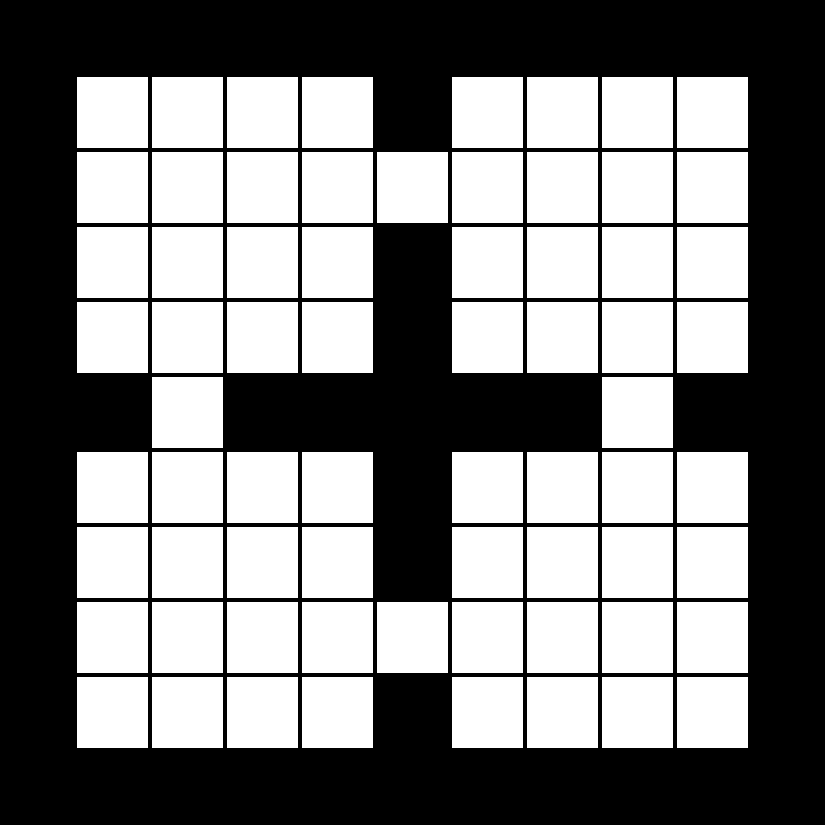
\includegraphics[width=0.48\columnwidth]{media/4-room-grid-world.pdf}
\hfill
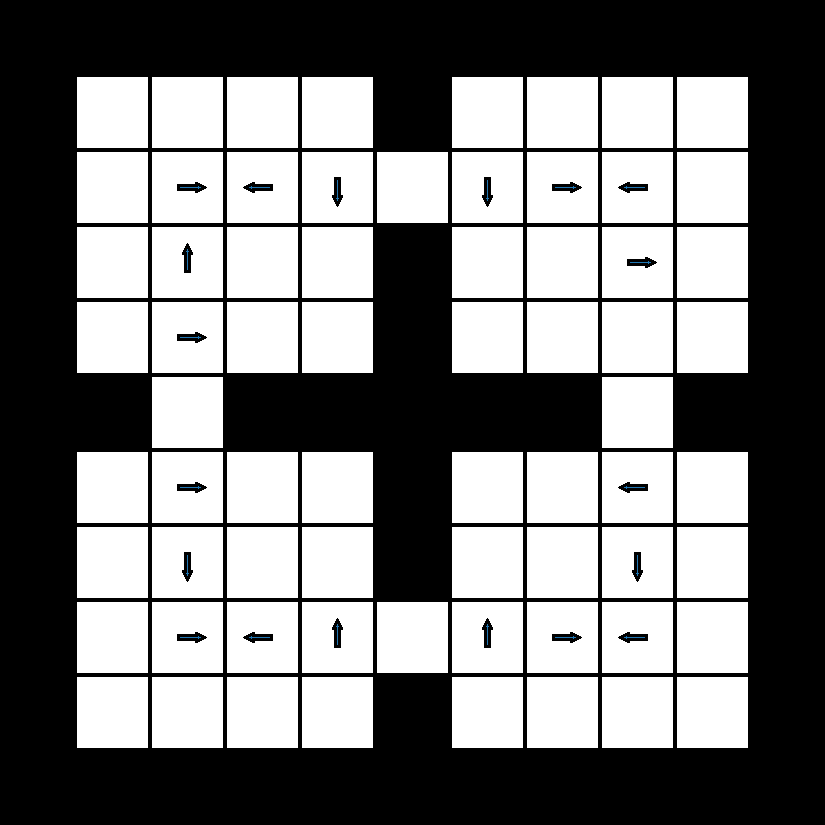
\includegraphics[width=0.48\columnwidth]{media/4-room-windy-world.pdf}%
\caption{Left: Four room grid world. Right: Four room windy grid world with wind direction shown by arrows. The windy pushes the agent in the direction of wind with 0.25 probability irrespective of the action taken.}
\label{fig:four-room-grid-world}%
\end{figure}%
%
